\documentclass[a4paper,12pt,twoside,openright]{report}
\usepackage[T1]{fontenc}
\usepackage[utf8]{inputenc}
\usepackage[english, italian]{babel}
\usepackage{lmodern}

\usepackage{amsmath,amssymb}
\renewcommand{\phi}{\varphi}

\usepackage[heightrounded]{geometry}
\usepackage{indentfirst,microtype}

\usepackage{graphicx}
\usepackage{caption}
\usepackage{subfig}

\usepackage{hyperref}
\hypersetup{hidelinks}

\title{Annotazioni}
\author{Dario Barone}
\date{\today}

\setcounter{secnumdepth}{3}
\setcounter{tocdepth}{3}

\begin{document}

\maketitle
\tableofcontents
\clearpage

\section{5 dimensioni}
\label{sec:5dim}

\subsection{Rho monodisperso}
\label{subsec:5dimrhomono}
La teoria per $ \rho $ monodisperso è già stata verificata da simulazioni numeriche, pertanto ne ho eseguite a mia volta al fine di verificare che il mio programma funzionasse correttamente.
\subsubsection{Simulazione singola}
\label{subsubsec:5dimrhomonosingle}
Ho eseguito simulazioni di $ \rho $ monodisperso inizialmente per $ N = 5 $, con $ 1 \le p \le 20 $.

In figura \ref{fig:oneshotn5rhomono} sono riportati alcuni dei grafici ottenuti con $ -0.9 \le \rho \le 1 $ che varia a step di $ 0.1 $.
\begin{figure}[ht]
	\centering
	\subfloat{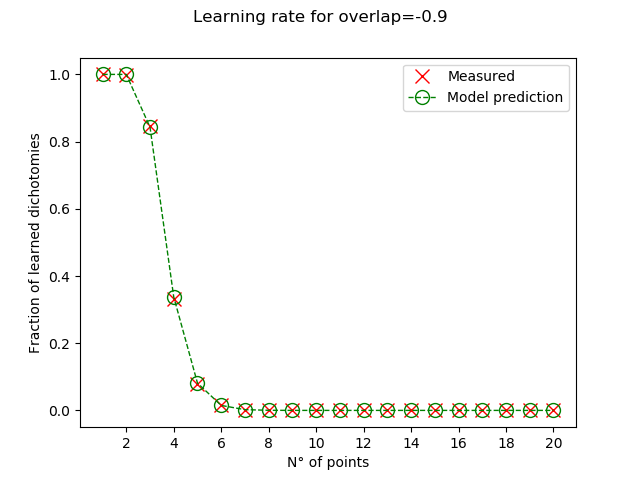
\includegraphics[width=0.3\textwidth]{immriassunto/oneshotn5rhomono/-0,9}}
	\subfloat{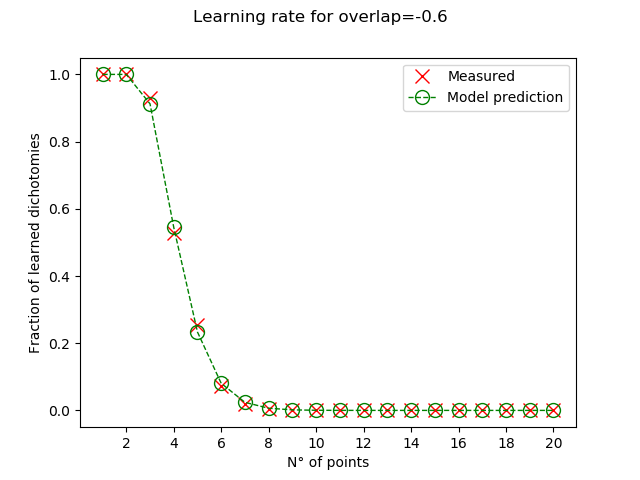
\includegraphics[width=0.3\textwidth]{immriassunto/oneshotn5rhomono/-0,6}}
	\subfloat{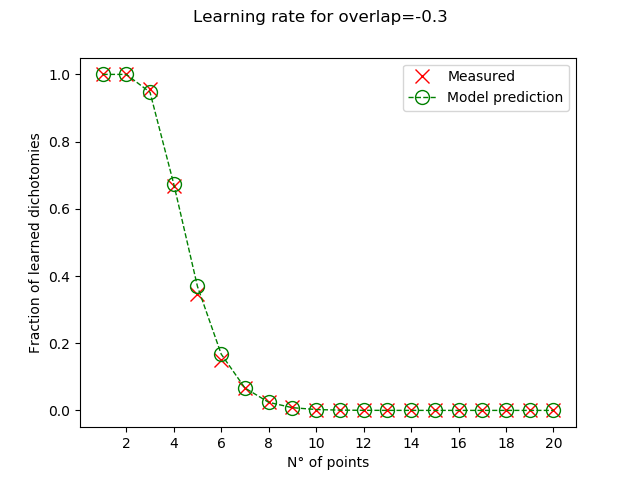
\includegraphics[width=0.3\textwidth]{immriassunto/oneshotn5rhomono/-0,3}}\newline
	\subfloat{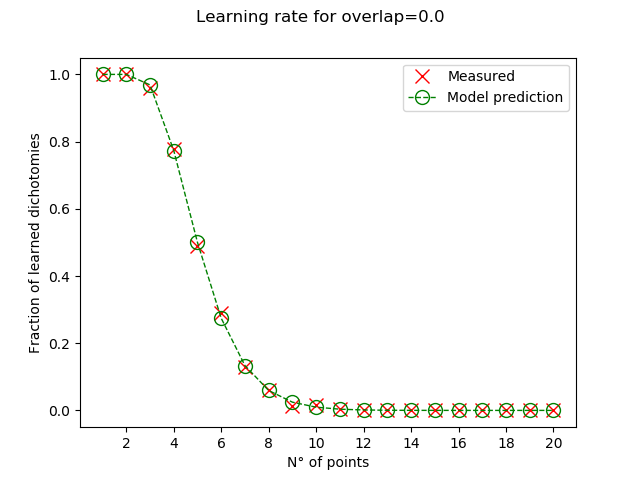
\includegraphics[width=0.3\textwidth]{immriassunto/oneshotn5rhomono/0,0}}
	\subfloat{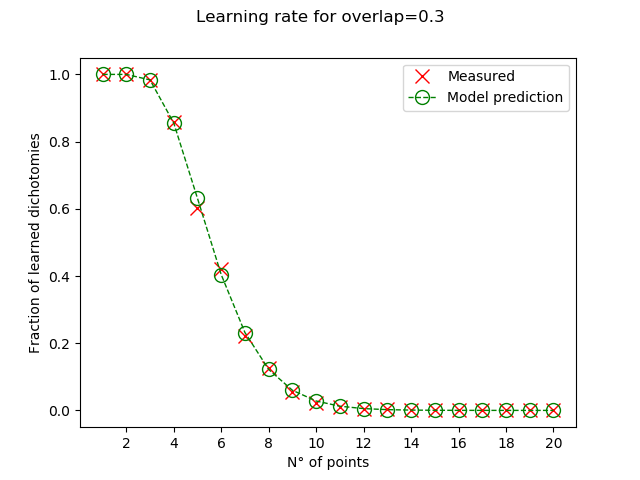
\includegraphics[width=0.3\textwidth]{immriassunto/oneshotn5rhomono/0,3}}
	\subfloat{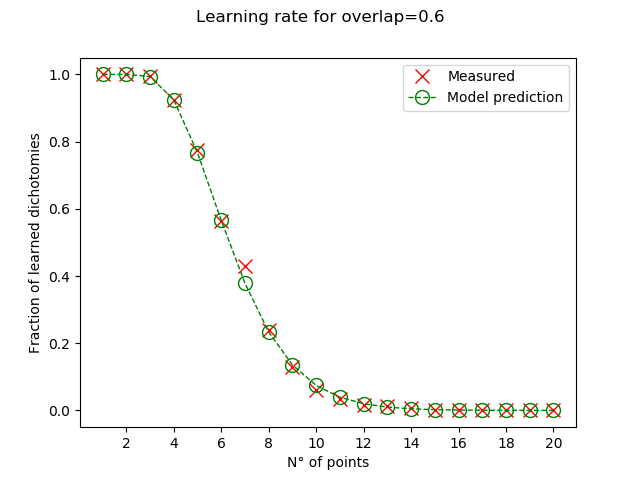
\includegraphics[width=0.3\textwidth]{immriassunto/oneshotn5rhomono/0,6}}
	\caption{}
	\label{fig:oneshotn5rhomono}
\end{figure}
Si nota che alcuni punti di discostano discretamente dal valore atteso. In particolare alcuni valori misurati sono maggiori di quelli attesi, altri sono minori, il che lascia pensare che gli errori siano di origine statistica.
Una conferma si può riscontrare nella simulazione con $ \rho = 1 $ (mostrato in figura \ref{fig:oneshotn5rhomono=1}, che corrisponde al caso in cui i punti del doppietto sono sovrapposti.
\begin{figure}[ht]
	\centering
	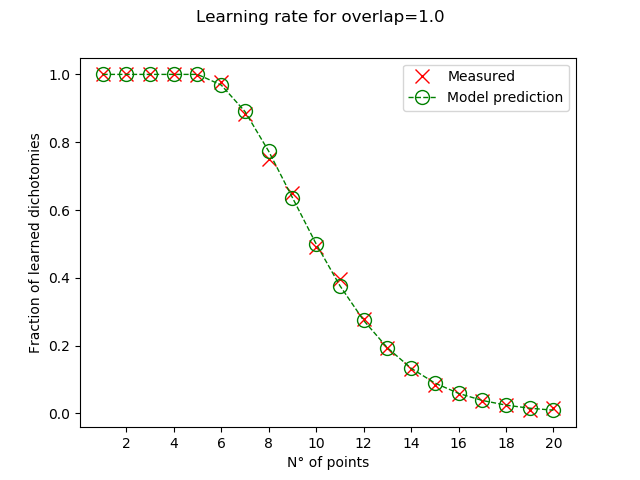
\includegraphics[width=0.5\textwidth]{immriassunto/oneshotn5rhomono/1,0}
	\caption{}
	\label{fig:oneshotn5rhomono=1}
\end{figure}
In questo caso infatti deve risultare che la simulazione sia perfettamente compatibile con le previsioni teoriche





\subsubsection{Simulazione con statistica}
\label{subsubsec:5dimrhomonostat}
Per i motivi sopra descritti, si è deciso di modificare la simulazione in modo tale che ognuno dei punti fosse in realtà la media su 10 ripetizioni.
In questo caso si è verificato che i valor medi fossero decisamente compatibili con le previsioni, tanto che il valore teorico rientrava sempre entro una $ \sigma $ (come $ \sigma $ si è considerata la deviazione standard della media delle $ 10 $ misure).
Si riportano in figura \ref{fig:statn5rhomono} i risultati di queste simulazioni, dove le barre d'errore sono state omesse nei grafici perchè poco significative.
\begin{figure}[ht]
	\centering
	\subfloat{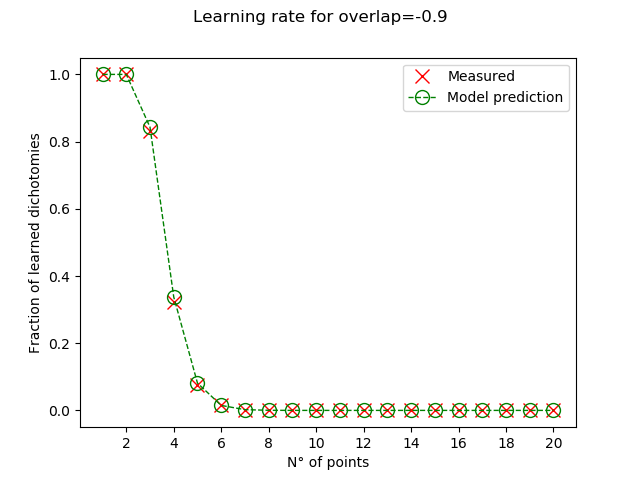
\includegraphics[width=0.3\textwidth]{immriassunto/statn5rhomono/-0,9}}
	\subfloat{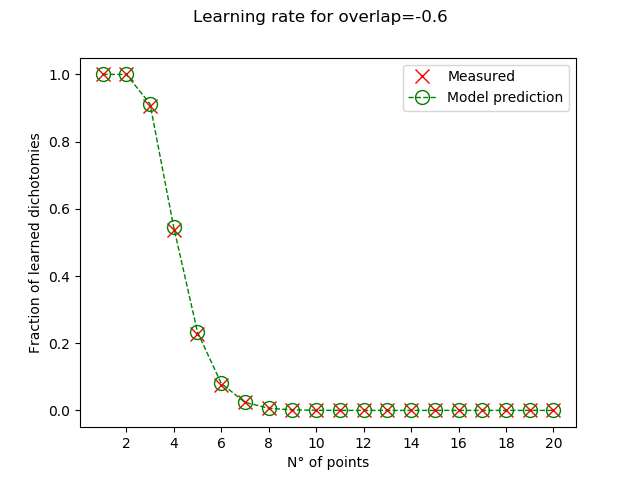
\includegraphics[width=0.3\textwidth]{immriassunto/statn5rhomono/-0,6}}
	\subfloat{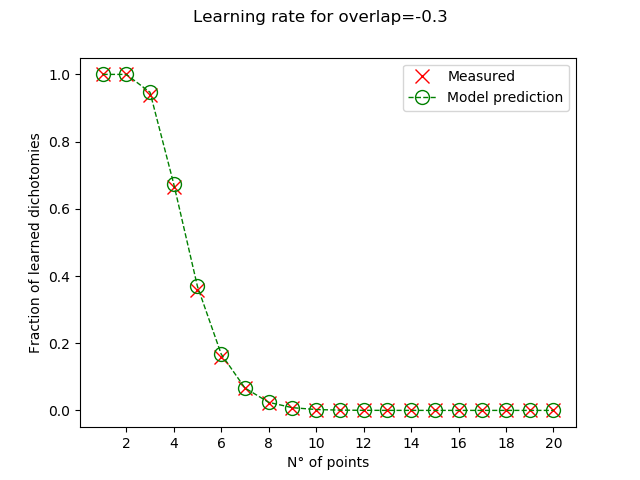
\includegraphics[width=0.3\textwidth]{immriassunto/statn5rhomono/-0,3}}\newline
	\subfloat{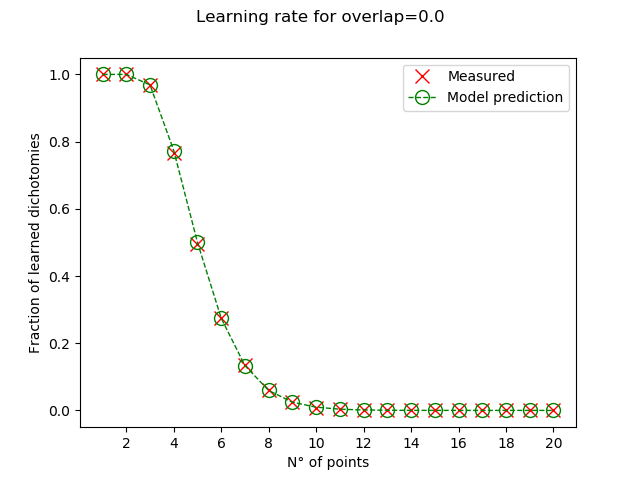
\includegraphics[width=0.3\textwidth]{immriassunto/statn5rhomono/0,0}}
	\subfloat{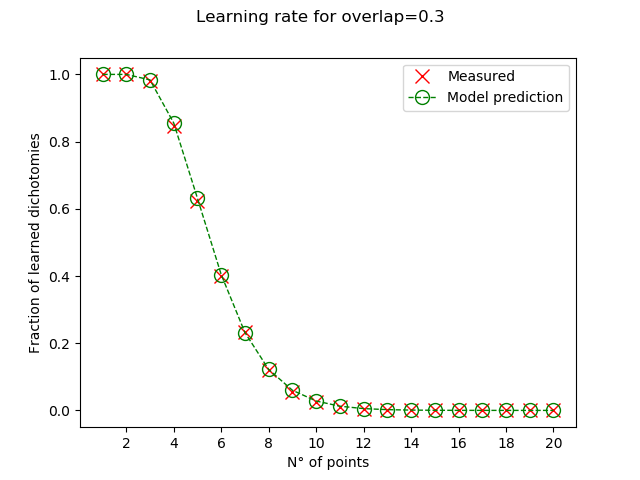
\includegraphics[width=0.3\textwidth]{immriassunto/statn5rhomono/0,3}}
	\subfloat{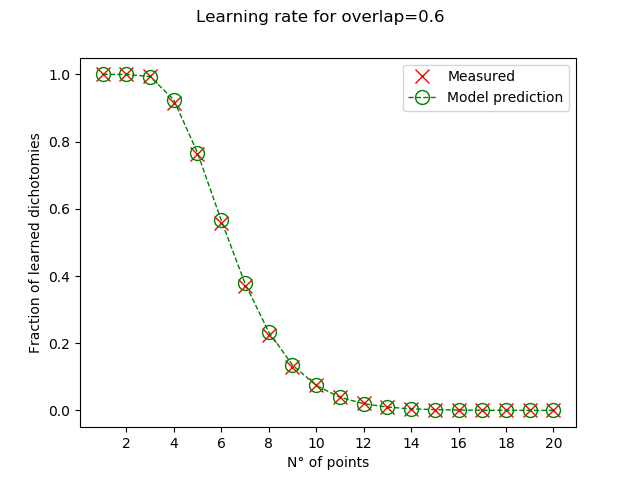
\includegraphics[width=0.3\textwidth]{immriassunto/statn5rhomono/0,6}}
	\caption{}
	\label{fig:statn5rhomono}
\end{figure}
Osservando i grafici si nota una certa sistematicità nell'errore: questo può essere attribuito al numero massimo di \emph{batches}, che talvolta impedisce al perceptron di portare a termine l'apprendimento.

Il grafico dell'errore (figura \ref{fig:errorn5rhomono}) al variare dell'overlap evidenzia, almeno per quanto riguarda la simulazione con statistica, che la discrepanza tra valore misurato e teorico è circa costante ed è di molto inferiore rispetto all'incertezza statistica. Sembra però che l'incertezza statistica tenda a crescere al crescere dell'overlap e non è ben chiaro perché.
\begin{figure}[ht]
	\centering
	\subfloat{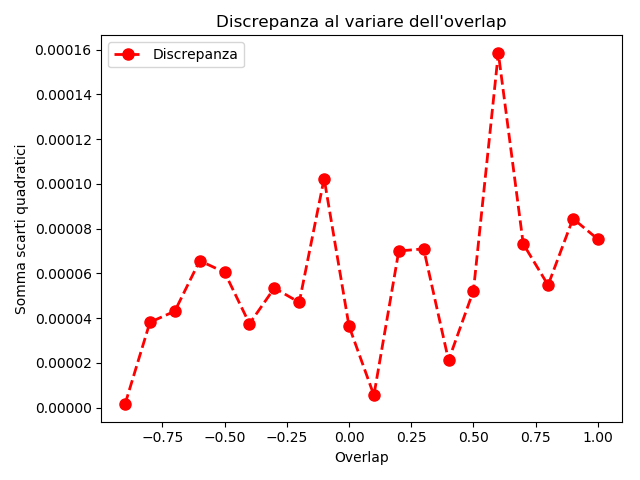
\includegraphics[width=0.5\textwidth]{immriassunto/oneshotn5rhomono/error}}
	\subfloat{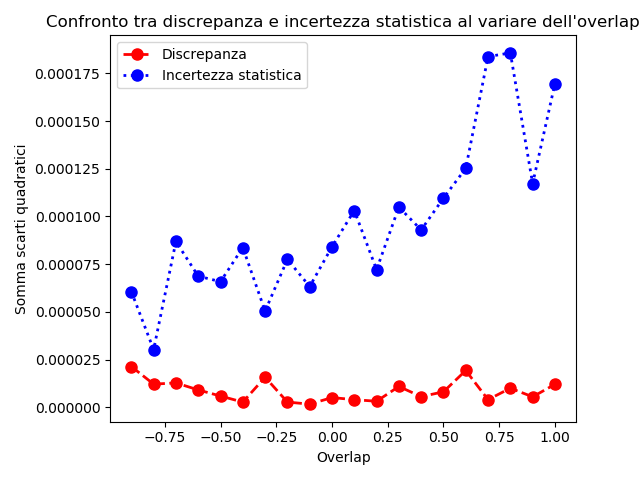
\includegraphics[width=0.5\textwidth]{immriassunto/statn5rhomono/error}}
	\caption{}
	\label{fig:errorn5rhomono}
\end{figure}



\subsection{Rho polidisperso}
\label{subsec:5dimrhopoli}
Si ha una buona evidenza del funzionamento del codice scritto per $ \rho $ monodisperso, pertanto si procede a simulare la polidispersione. In questo caso, con "polidispersione" si intende una $ \rho $ che può assumere due distinti valori, dapprima con stesso peso (vedi \ref{subsubsec:5dimrhopolisame}) e in seguito con pesi distinti (vedi \ref{subsubsec:5dimrhopolidiff}).

Si è trattato sia il caso di simulazione singola, per verificare che tutto funzionasse correttamente, sia il caso con statistica. Qui riporto solamente il caso con statistica visto che il caso singolo è risultato soddisfacente.

Le previsioni teoriche sono state effettuate nell'ipotesi che valga il \emph{mean-field}, ossia che la legge che determina $C_{n,p}$ per $\rho$ monodisperso valga anche nel caso di polidispersione a patto che si usi come valore di $\Psi$ il valor medio di $\Psi(\rho)$.

\subsubsection{Simulazione con pesi uguali}
\label{subsubsec:5dimrhopolisame}
Si riportano qui solo alcuni grafici di esempio (figura \ref{fig:samen5rhopoli}), tenendo conto che di nuovo si sono svolte simulazioni per $ -0.9 \le \rho_1 \le 1 $ e $ \rho_1 \le \rho_2 \le 1 $ sempre a step di $0.1$ (per un totale di $210$ simulazioni), dove però molte di queste sono del tutto simili tra loro.
\begin{figure}[ht]
	\centering
	\subfloat{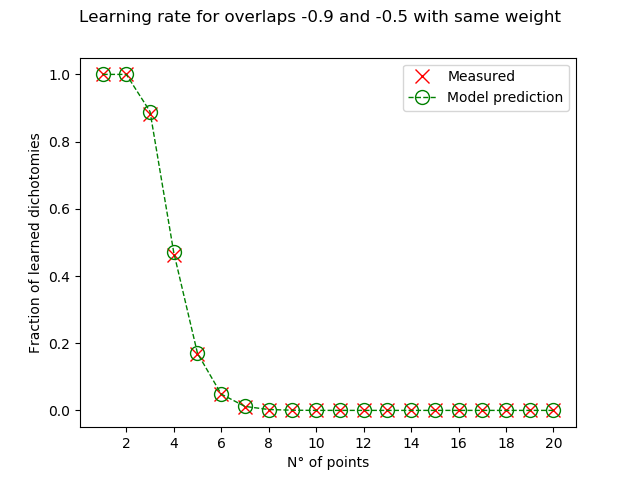
\includegraphics[width=0.3\textwidth]{immriassunto/statn5rhopolisame/-0,9;-0,5}}
	\subfloat{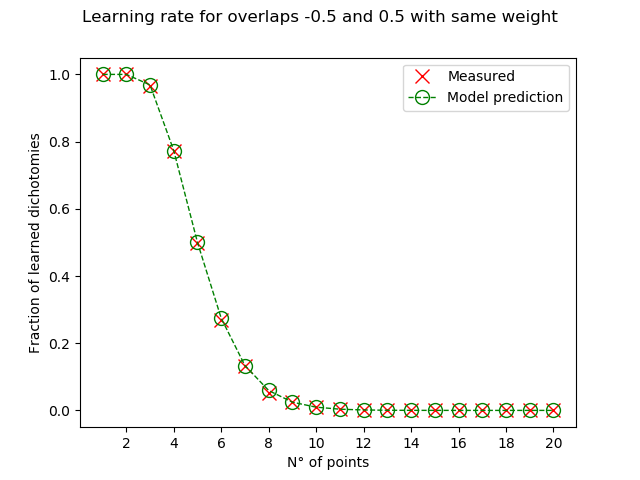
\includegraphics[width=0.3\textwidth]{immriassunto/statn5rhopolisame/-0,5;0,5}}
	\subfloat{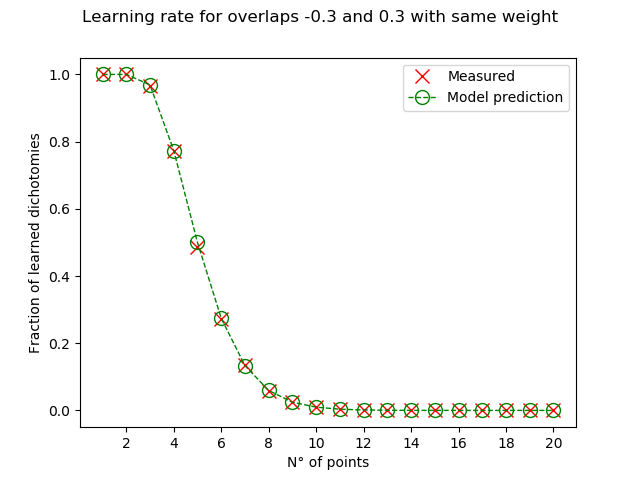
\includegraphics[width=0.3\textwidth]{immriassunto/statn5rhopolisame/-0,3;0,3}}\newline
	\subfloat{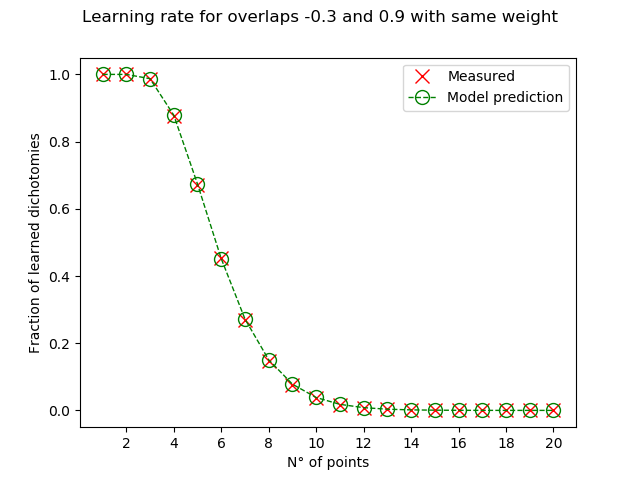
\includegraphics[width=0.3\textwidth]{immriassunto/statn5rhopolisame/-0,3;0,9}}
	\subfloat{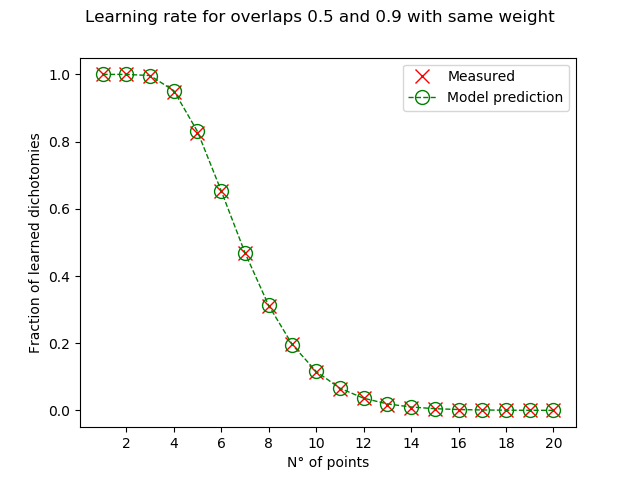
\includegraphics[width=0.3\textwidth]{immriassunto/statn5rhopolisame/0,5;0,9}}
	\subfloat{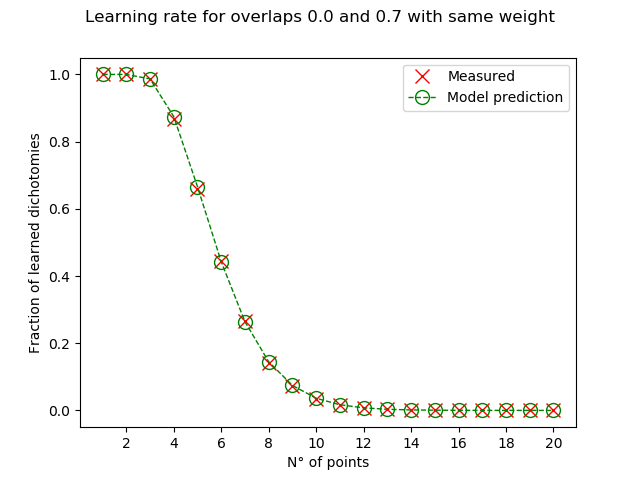
\includegraphics[width=0.3\textwidth]{immriassunto/statn5rhopolisame/0,0;0,7}}
	\caption{}
	\label{fig:samen5rhopoli}
\end{figure}
Come si può notare, tutti i grafici hanno un'ottima compatibilità con le predizioni teoriche effettuate nell'ipotesi di \emph{mean-field}. 

Si riportano anche i grafici riportanti la discrepanza e l'incertezza statistica (figura \ref{fig:errorsamen5rhopoli}).
\begin{figure}[!ht]
	\centering
	\subfloat{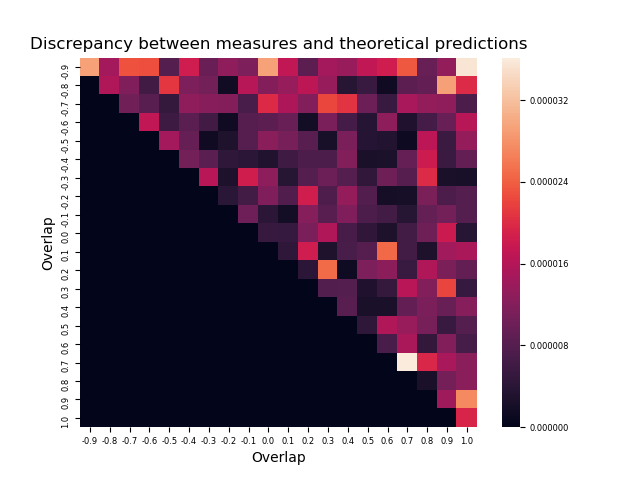
\includegraphics[width=0.5\textwidth]{immriassunto/statn5rhopolisame/Heatmap_discrepancy}}
	\subfloat{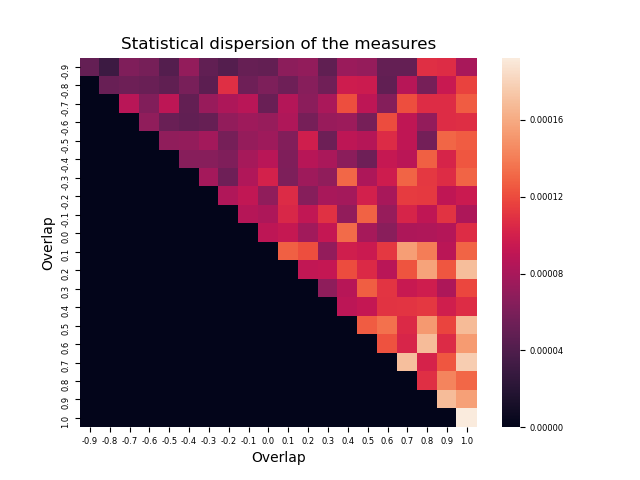
\includegraphics[width=0.5\textwidth]{immriassunto/statn5rhopolisame/Heatmap_statistical}}
	\caption{}
	\label{fig:errorsamen5rhopoli}
\end{figure}
Dal grafico della discrepanza si può constatare che la essa sembra essere distribuita casualmente, senza una correlazione evidente con i valori di $\rho$, fatta eccezione per valori molto bassi ($ \rho \le -0.7 $) dove sembra che la discrepanza sia più marcata.
Nel grafico dell'incertezza statistica, invece, appare evidente un certo pattern: all'aumentare del valor medio di $\rho$, aumenta anche l'incertezza statistica.

Entrambe le considerazioni confermano le osservazioni fatte precedentemente per $\rho$ monodisperso. Inoltre si può osservare che i valori assoluti di discrepanza e errore statistico sono dello stesso ordine di grandezza per $\rho$ monodisperso e polidisperso.

\subsubsection{Simulazione con pesi diversi}
\label{subsubsec:5dimrhopolidiff}
Si riportano qui solo alcuni grafici di esempio (figura \ref{fig:diffn5rhopoli}), tenendo conto che di nuovo si sono svolte simulazioni per $ -0.9 \le \rho_1 \le 1 $ e $ -0.9 \le \rho_2 \le 1 $ sempre a step di $0.1$ (per un totale di $400$ simulazioni), dove però molte di queste sono del tutto simili tra loro. In questo caso si è considerato $p(\rho_1)=2\,p(\rho_2)$, pertanto non è equivalente scambiare i due valori di $\rho$.
\begin{figure}[ht]
	\centering
	\subfloat{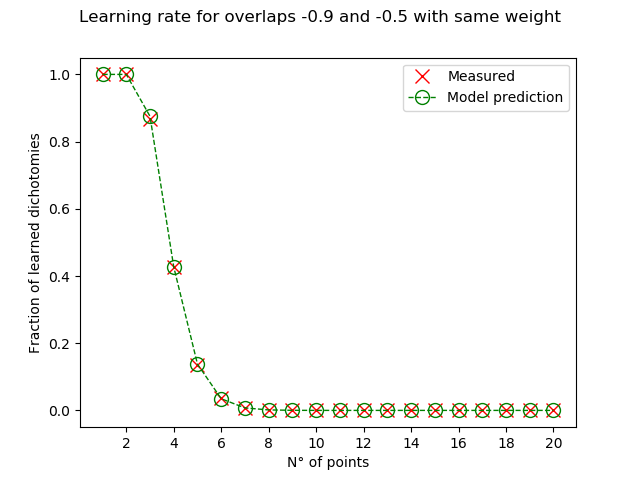
\includegraphics[width=0.3\textwidth]{immriassunto/statn5rhopolidiff/-0,9;-0,5}}
	\subfloat{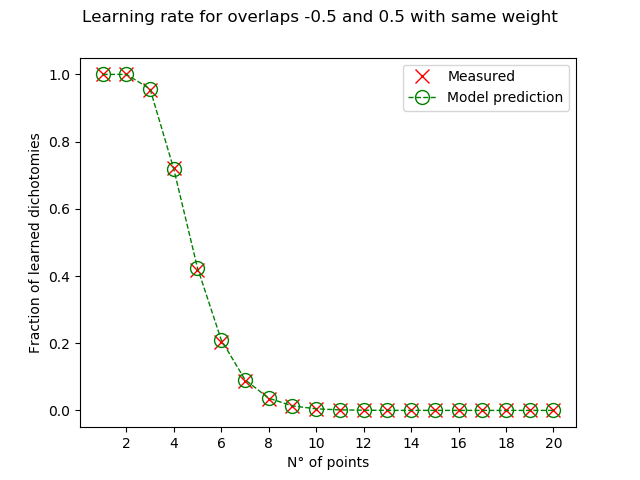
\includegraphics[width=0.3\textwidth]{immriassunto/statn5rhopolidiff/-0,5;0,5}}
	\subfloat{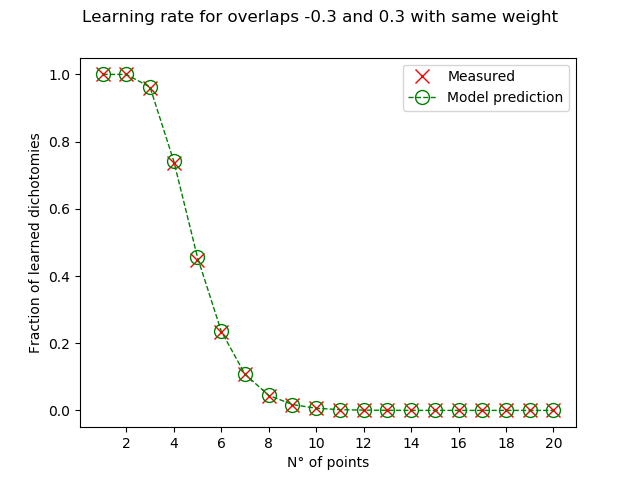
\includegraphics[width=0.3\textwidth]{immriassunto/statn5rhopolidiff/-0,3;0,3}}\newline
	\subfloat{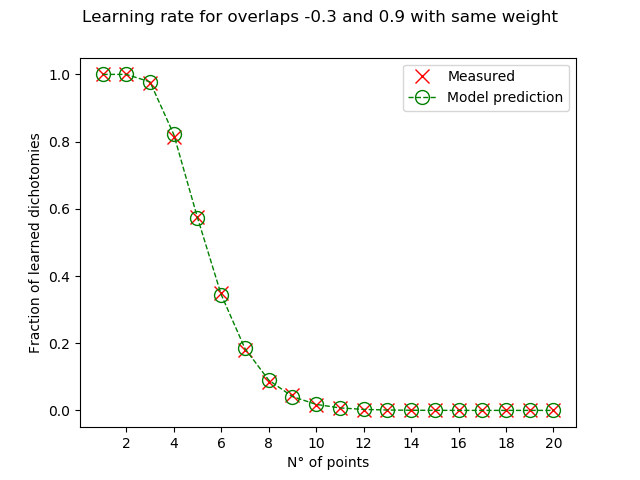
\includegraphics[width=0.3\textwidth]{immriassunto/statn5rhopolidiff/-0,3;0,9}}
	\subfloat{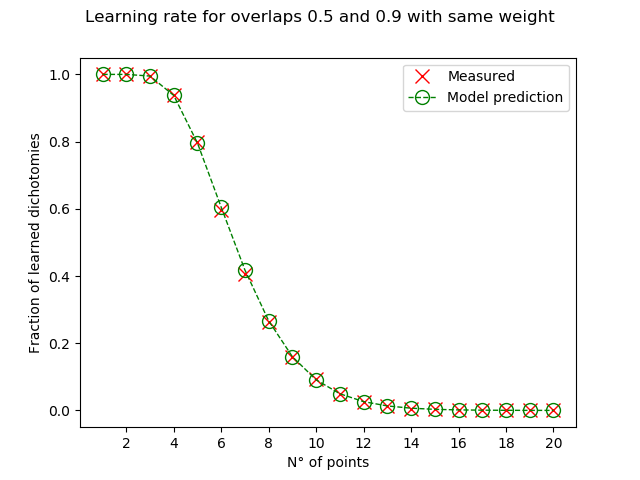
\includegraphics[width=0.3\textwidth]{immriassunto/statn5rhopolidiff/0,5;0,9}}
	\subfloat{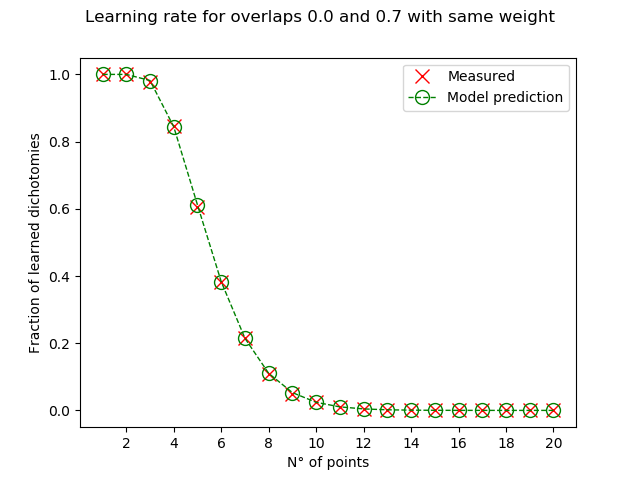
\includegraphics[width=0.3\textwidth]{immriassunto/statn5rhopolidiff/0,0;0,7}}
	\caption{}
	\label{fig:diffn5rhopoli}
\end{figure}

Si riportano anche heatmaps relative alla discrepanza e all'incertezza statistica che a priori non devono essere simmetriche (figura \ref{fig:errordiffn5rhopoli}).
\begin{figure}[!ht]
	\centering
	\subfloat{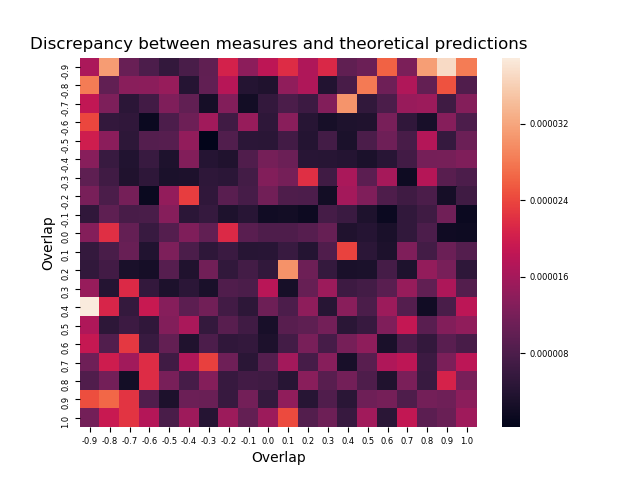
\includegraphics[width=0.5\textwidth]{immriassunto/statn5rhopolidiff/Heatmap_discrepancy}}
	\subfloat{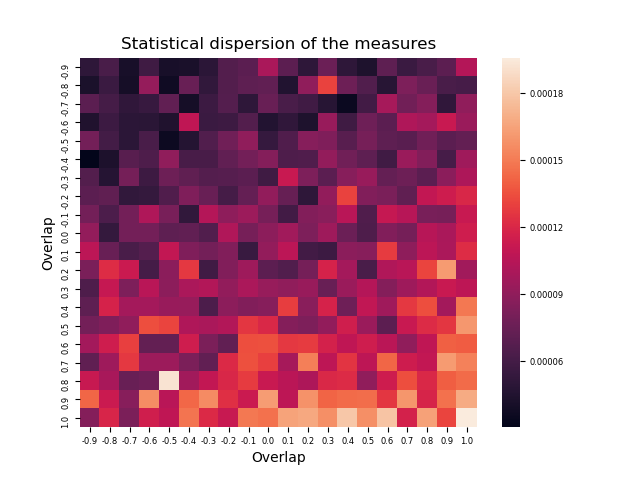
\includegraphics[width=0.5\textwidth]{immriassunto/statn5rhopolidiff/Heatmap_statistical}}
	\caption{}
	\label{fig:errordiffn5rhopoli}
\end{figure}
Anche qui valgono le considerazioni fatte precedentemente per polidispersione con stessi pesi


\subsection{Rho gaussiano}
\label{subsec:5dimrhogauss}

Ho cominciato a fare le simulazioni con $\rho$ distribuito secondo gaussiana. Per qualsiasi $\mu$ e $\sigma$ bassi, i risultati sono buoni (figura \ref{fig:gaussn5}), nei casi con $\sigma$ elevati ho sbagliato la simulazione e sto aspettando i dati corretti.

\begin{figure}[ht]
	\centering
	\subfloat{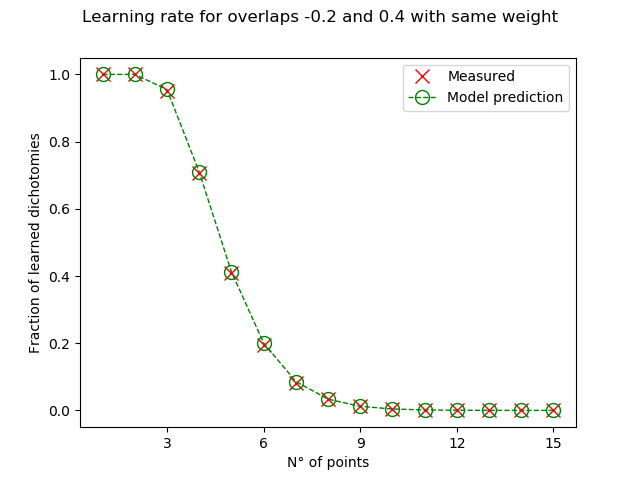
\includegraphics[width=0.5\textwidth]{immriassunto/statn5rhogauss/-0,2;0,4}}
	\subfloat{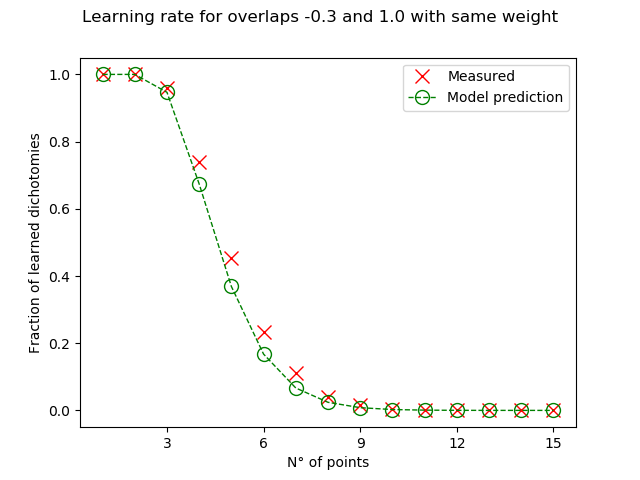
\includegraphics[width=0.5\textwidth]{immriassunto/statn5rhogauss/-0,3;1,0}}\newline
	\subfloat{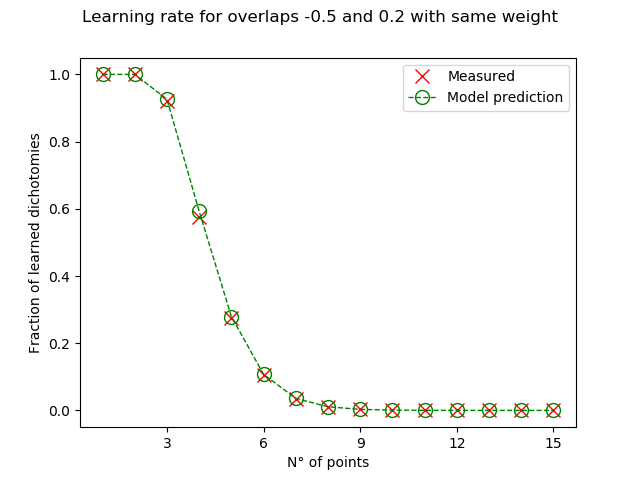
\includegraphics[width=0.5\textwidth]{immriassunto/statn5rhogauss/-0,5;0,2}}
	\subfloat{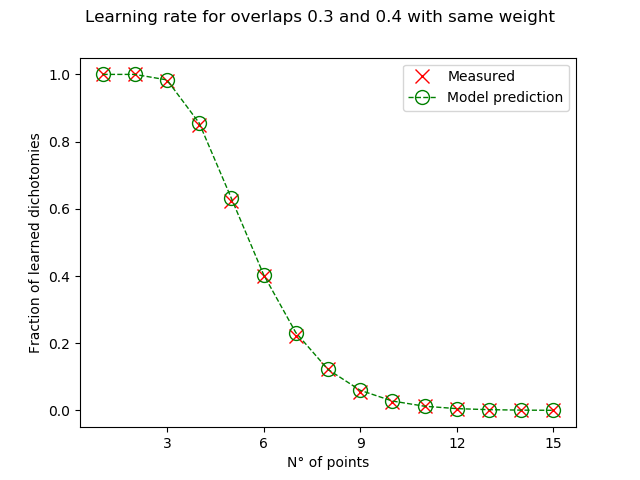
\includegraphics[width=0.5\textwidth]{immriassunto/statn5rhogauss/0,3;0,4}}
	\caption{}
	\label{fig:gaussn5}
\end{figure}




\section{Più dimensioni}
\label{sec:piùdim}

\subsection{Dimensione 10}
\label{subsec:10dim}

Per generalizzare i risultati ottenuti si sono eseguite simulazioni anche in N=10, ma, poichè le simulazioni erano molto più lunghe, si è deciso di ridurre il numero di punti massimi a $ p_\textup{max} = 3\,N $ e di diradarli in modo che venga sondato un punto ogni due.

\subsubsection{Rho monodisperso}
\label{subsubsec:10dimrhomono}
Si riportano i grafici (dati in figura \ref{fig:n10rhomono} e errori in figura \ref{fig:errorn10rhomono}) corrispondenti a quelli mostrati per $5$ dimensioni
\begin{figure}[ht]
	\centering
	\subfloat{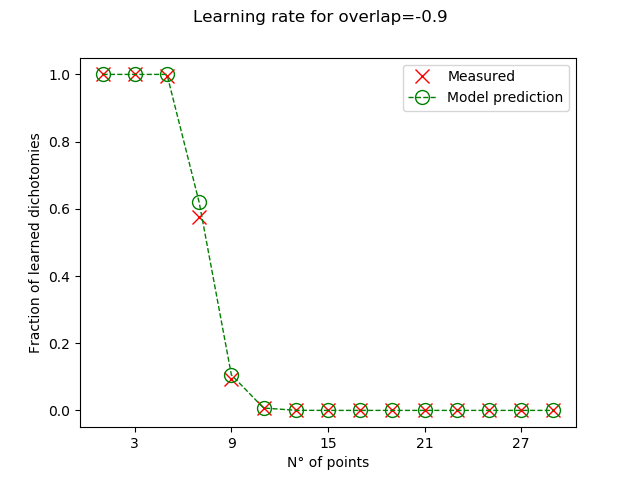
\includegraphics[width=0.3\textwidth]{immriassunto/statn10rhomono/-0,9}}
	\subfloat{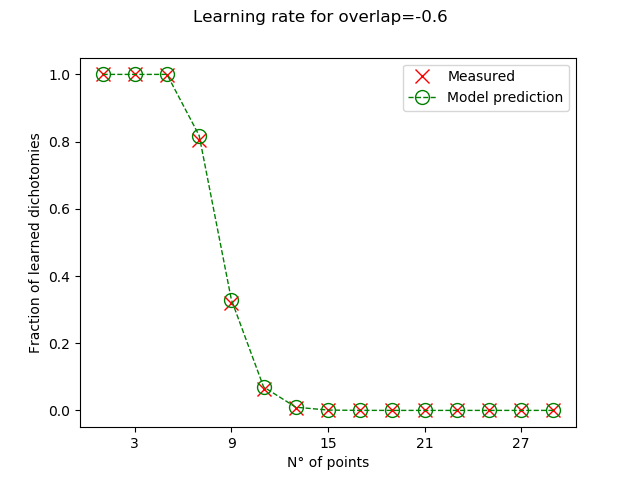
\includegraphics[width=0.3\textwidth]{immriassunto/statn10rhomono/-0,6}}
	\subfloat{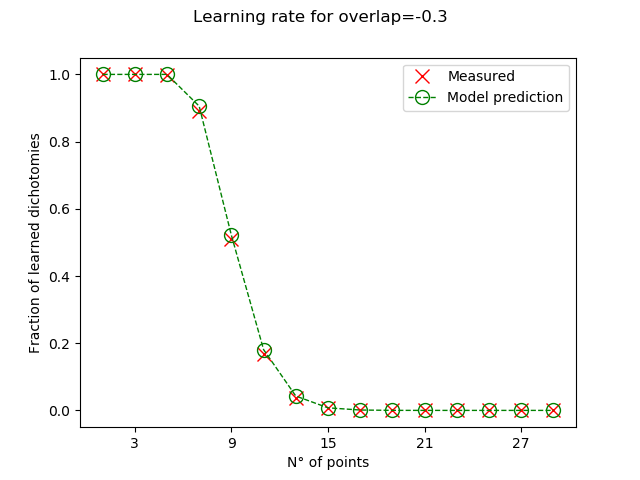
\includegraphics[width=0.3\textwidth]{immriassunto/statn10rhomono/-0,3}}\newline
	\subfloat{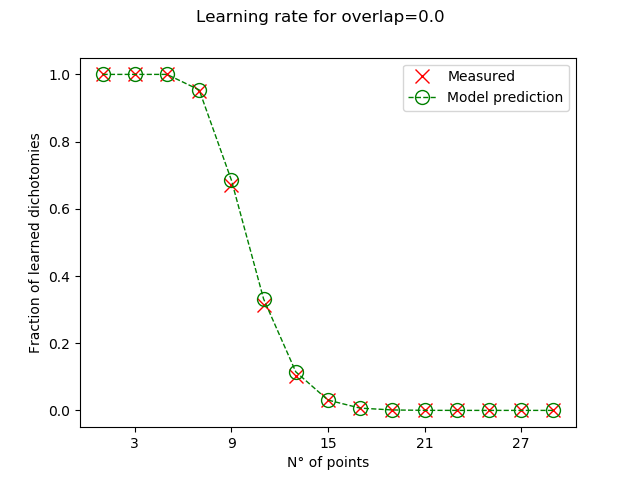
\includegraphics[width=0.3\textwidth]{immriassunto/statn10rhomono/0,0}}
	\subfloat{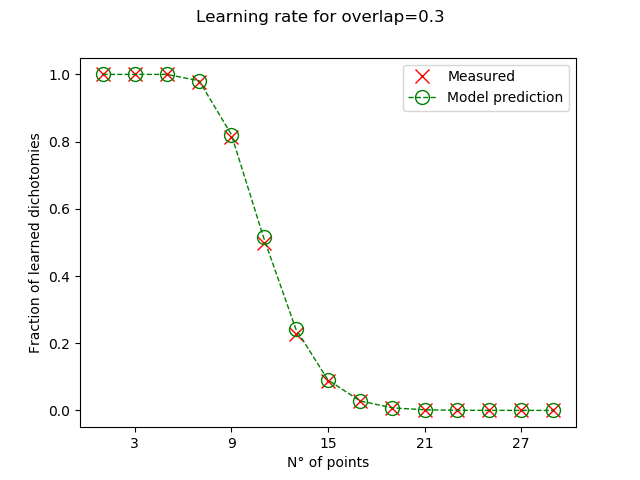
\includegraphics[width=0.3\textwidth]{immriassunto/statn10rhomono/0,3}}
	\subfloat{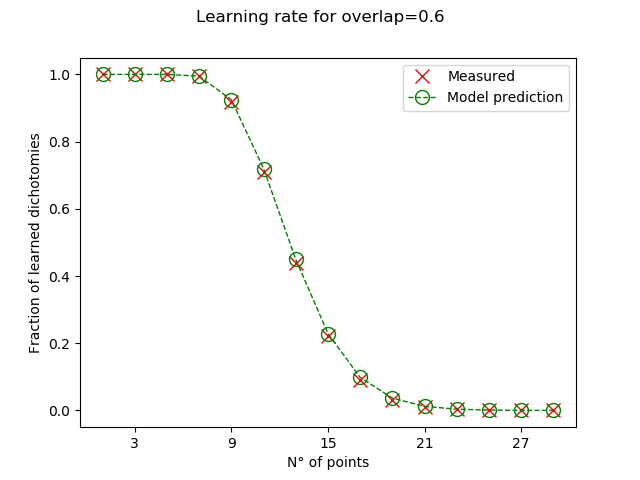
\includegraphics[width=0.3\textwidth]{immriassunto/statn10rhomono/0,6}}
	\caption{}
	\label{fig:n10rhomono}
\end{figure}
\begin{figure}[!ht]
	\centering
	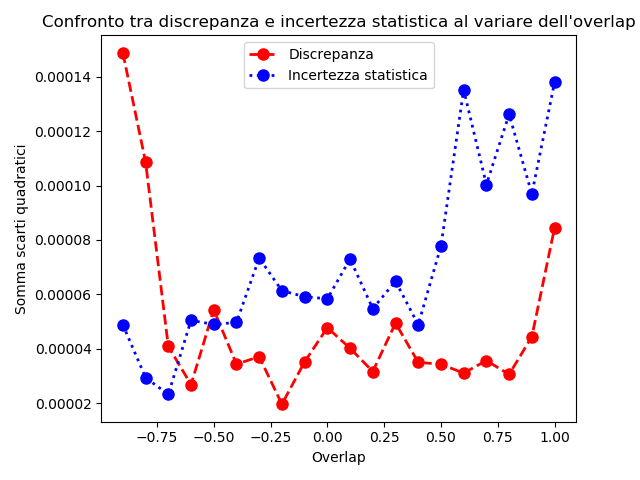
\includegraphics[width=0.5\textwidth]{immriassunto/statn10rhomono/error}
	\caption{}
	\label{fig:errorn10rhomono}
\end{figure}
Si possono confermare le osservazioni su $5$ dimensioni per cui l'incertezza statistica aumenta all'aumentare di $\rho$. Si conferma anche il fatto che la discrepanza è all'incirca costante fatta eccezione per valori di $\rho$ molto bassi, dove la discrepanza in questo caso è notevole e per niente compatibile con l'incertezza statistica. Occorre però notare che le discrepanze per tutti i valori di $\rho$ sono maggiori rispetto al caso di $5$ dimensioni. Questo si potrebbe spiegare col fatto che aumentando le dimensioni, sia necessario un numero massimo di \emph{batches} più alto per permettere al perceptron di imparare le dicotomie.


\subsubsection{Rho polidisperso}
\label{subsubsec:10dimrhopoli}
In attesa della simulazione


\subsection{Dimensione 20}
\label{subsec:20dim}
Per generalizzare i risultati ottenuti si sono eseguite simulazioni anche in N=10, ma, poichè le simulazioni erano molto più lunghe, si è deciso di ridurre il numero di punti massimi a $ p_\textup{max} = 3\,N $ e di diradarli in modo che venga sondato un punto ogni quattro. Le simulazioni con dimensione $20$ potrebbero anche confermare l'ipotesi che la crescente discrepanza sia sistematica dovuta al numero finito di \emph{batches}.

In attesa della simulazione


\section{Considerazioni varie e possibili sviluppi}
\begin{itemize}
	\item Devo ancora capire bene come si comporta la complessità dell'algoritmo in funzione del numero di dimensioni.
	\item Sarebbe utile per fare più simulazioni ma la loro complessità computazionale richiede di ``tagliare'' qualcosa. Alcune ipotesi sono:
	\begin{enumerate}
		\item diminuire la statistica (ma 10 ripetizioni credo sia il minimo sindacabile)
		\item diminuire il valore massimo di punti $p_\textup{max}$ che si indaga perchè la curva è quasi sempre piatta verso la fine
		\item avere punti più diradati (ma implica rifare le simulazioni)
	\end{enumerate}
	\item Si potrebbe aggiungere qualche studio riguardo la capacità del perceptron (richiede di rifare le simulazioni).
	\item Forse può aver senso confrontare la varianza misurata di $C_{n,p}$ con quella che si può ricavare utilizzando la varianza di $\Psi$.
	\item I grafici sono alcuni in inglese e alcuni in italiano. Il programma è scritto (nomi variabili) e commentato in inglese, ma la tesi in italiano. È meglio quindi scrivere in italiano sui grafici credo
	\item Al momento le simulazioni per $N=5$ procedono punto per punto, mentre le simulazioni con $N=10$ e $N=20$ procedono ogni $2$ e $4$ punti, ma partono da $1$ e quindi si sballano i multipli. Trascuro o sistemo?
	\item Riguardo le simulazioni con $\rho$ distribuito in modo gaussiano, quali sono i valori di $\mu$ e $\sigma$ sensati da simulare? E soprattutto quanto dev'essere la minima statistica che si deve effettuare?
\end{itemize}

\end{document}